%Example of use of oxmathproblems latex class for problem sheets
\documentclass{oxmathproblems}
\usepackage{hyperref}
\usepackage[ngerman]{babel}
\usepackage{subfig}
%(un)comment this line to enable/disable output of any solutions in the file
%\printanswers

%define the page header/title info
\oxfordterm{26.06.2021}
\course{Vorlesung: DS-ML-PL SS21}
\sheetnumber{2}
\sheettitle{Güte von Äpfeln} %can leave out if no title per sheet

% add further contact details to footer if desired,
%e.g. email address, or name and email address
\contact{Juan Arango: ara@biba.uni-bremen.de, Nicolas Jathe: jat@biba.uni-bremen.de}


\begin{document}
\begin{questions}
\miquestion
Eine Verpackungsanlage für Äpfel soll automatisiert werden. Für die geplante Automatisierung der Anlage muss entschieden werden, welche Äpfel noch verkaufbar sind. Dieser Schritt soll von einer Kamera und einer Auswerteeinheit übernommen werden. Nutzen Sie die aus der Vorlesung bekannten Methoden um eine Klassifikation der Bilder aus dem Datensatz \url{https://data.ips.biba.uni-bremen.de/Lehre/dsmlpl_SS21/Apples_Defect_Healthy.tgz} vorzunehmen. Im StudIP finden Sie ein Notebook, welches Sie als Grundlage nutzen können. 
\begin{parts}
  \part Unterteilen Sie die Daten selbstständig in Training- und Testdaten.
  \part Nutzen Sie die \texttt{parent\textunderscore label}-Funktion um die Bilder der Trainingsdaten einer Klasse zuzuordnen.  
  \part Erstellen Sie ein eigenes Neuronales Netz oder nutzen Sie ein vorgefertigtes und trainieren Sie es entsprechend der Klassifikationsaufgabe.
  \part Überprüfen Sie die Performance Ihrer Lösung auf den Testdaten.
\end{parts}

\begin{solution}
  The solution would go here
\end{solution}

\begin{figure}%
    \centering
    \subfloat[][\centering Sortiereinheit]{{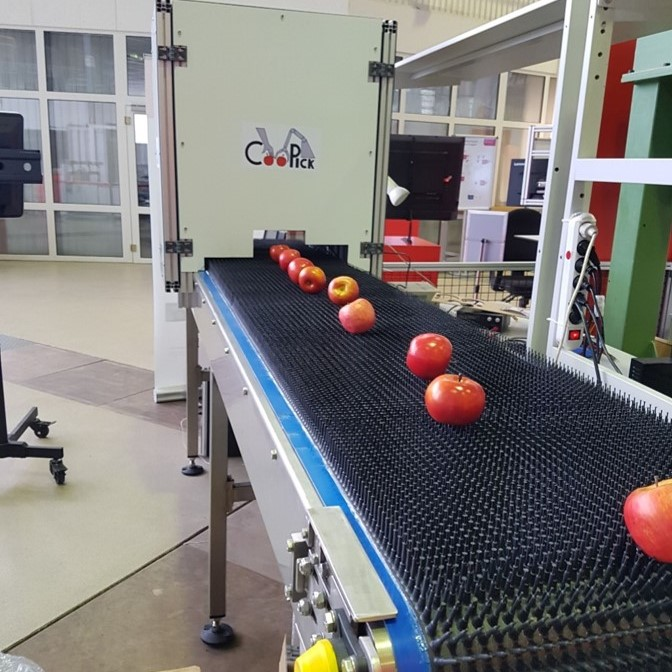
\includegraphics[width=4cm]{coopickq.jpg}}}
    \qquad
    \subfloat[][\centering Guter Apfel]{{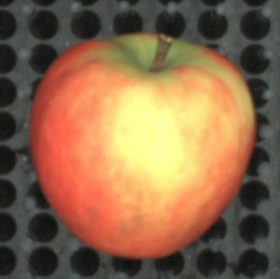
\includegraphics[width=4cm]{guterapfel.png}}}
    \qquad
    \subfloat[][\centering Schlechter Apfel]{{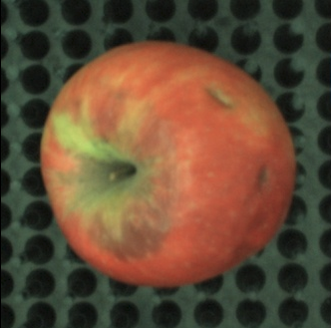
\includegraphics[width=4cm]{defekterapfel.png}}}
    %\caption{2 Figures side by side}%
    \label{fig:example}%
\end{figure}

\begin{solution}
  The solution would go here
\end{solution}
\end{questions}

\end{document}
